\documentclass{article}
\usepackage{fontspec}
\usepackage{polyglossia}
\setdefaultlanguage{french}
\usepackage[a4paper,margin=3cm]{geometry}

\usepackage{amsmath}
\usepackage{amssymb}
\usepackage{array}
\usepackage{auto-pst-pdf}
\usepackage{booktabs}
\usepackage{cite}
\usepackage{graphicx}
\usepackage{lmodern}
\usepackage{marvosym}
\usepackage{mathrsfs}
\usepackage{minted}
\usepackage{multicol}
\usepackage{multirow}
\usepackage{paralist}
\usepackage{schemabloc}
\usepackage{siunitx}
\usepackage{soul}
\usepackage{tikz}
\usepackage[european,cuteinductors,siunitx]{circuitikz}
\usepackage{url,hyperref}
\usepackage{verbatim}
\usepackage{xunicode,xltxtra}

\title{
\includegraphics{../../../images/inp-enseeiht} \\ ~ \\ ~ \\ ~ \\ ~ \\ Rapport du BE Acceleromètre}
\author{François Pierron \& Guilhem Saurel}
\date{\oldstylenums{3 février 2014}}

\begin{document}

\begin{titlepage}
    \setcounter{page}{0}
    \maketitle
    \vfill
    \tableofcontents
    \thispagestyle{empty}
\end{titlepage}

\section*{Introduction}

L’objectif de ce BE est de concevoir une chaîne d’instrumentation composée d’un accéléromètre MEMS qui nous donne une capacité variable en fonction de l’accélération, suivi d’un système qui transforme cette information en une tension proportionelle.

~

Le MEMS étant fourni, nous allons devoir concevoir et simuler un amplificateur ayant une entrée et une sortie différentielle, présentant un circuit de compensation du mode commun.


\includegraphics[width=\linewidth]{5_11.jpe}

\section{Architecture}

Pour faire notre «Fully Differential Amplifier» (FDA), nous partons sur les bases d’un amplificateur différentiel classique et nous ajoutons un second étage de sortie symétrique au premier.

~

Il faut alors revoir un peu la charge active, vu qu’elle n’était pas symétrique initialement, et nous optons pour un miroir de courrant piloté par une entrée externe, qui nous servira à reboucler le système pour anticiper le «Common Mode FeedBack» (CMFB).

\begin{centering}
    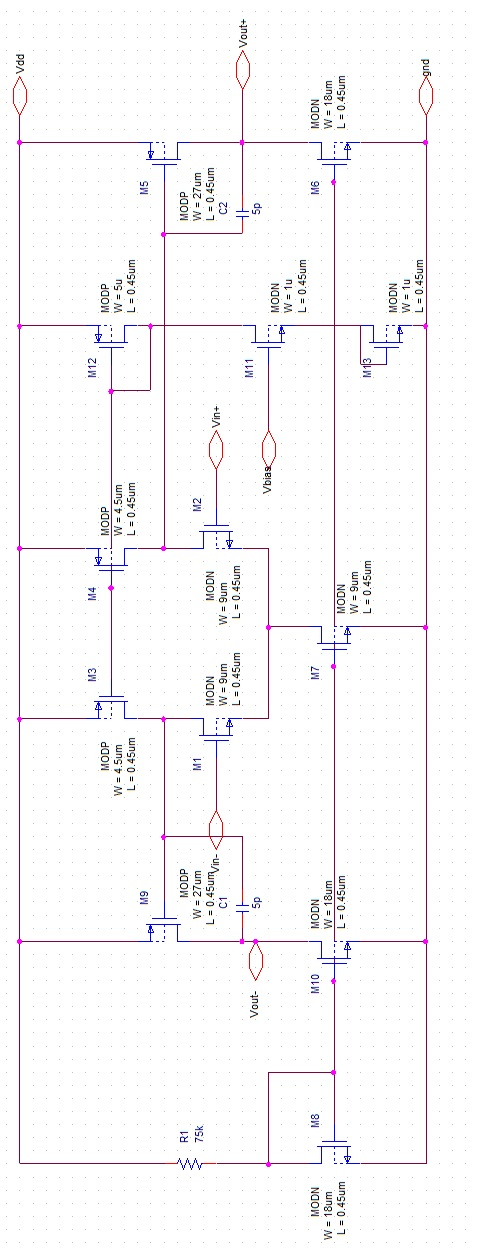
\includegraphics[height=25cm]{schema_diff.png}
\end{centering}

\section{Valeur de la capacité intégrée pour une sensibilité de 1V/g}

Ce système dans son ensemble sert à donner une information sur la tension de sortie qui doit être proportionelle à l’accélération, dont le coefficient de proportionnalité doit être d’1 V/g, soit $\cfrac{1 V}{9.81 m\cdot s^{-2}}$.

~

La sensibilité du MEMS est de 12 fF/g par capacité, sachant qu’il y en a deux vues en parallèle, pour une sortie à 1.65V.

On a donc une charge de $12\times2\times1.65=39.6$ fC pour une accélération de 1g. Si on veut que cette charge corresponde à une tension de 1V, il nous faut simplement une capacité de 39.6 fF.

~

Le calcul nous donne donc 39.6fF, cependant, après simulations, on se rend compte qu’une valeur de 44.2fF correspond mieux.
Cette différence de 10\% entre la valeur théorique et la valeur pratique déterminée par la simulation est probablement dûe aux capacités parasites dans le second étage de l’amplificateur différentiel.

\section{Intérêt d’un circuit de CMFB}

L’intérêt d’un circuit de CMFB est de fermer la boucle, tout en supprimant la tension différentielle de sortie. En effet, on ne peut pas fermer la boucle en utilisant le mode différentiel dans le cas d’un FDA.

~

Plusieurs solutions sont envisageables pour arriver à cet objectif. Nous allons commencer par la première qui vient à l’idée: faire une moyenne des tensions de sorties à l’aide de deux résistances identiques, et amplifier la différence de cette tension avec la tension de sortie désirée (1.65V) avant de la reboucler vers la charge active de la paire différentielle.

~

Au niveau schématique, on met ajoute alors ce CMFB dans un niveau hiérarchique supérieur à l’amplificateur différentiel et inférieur à la plupart de nos autres simulations :

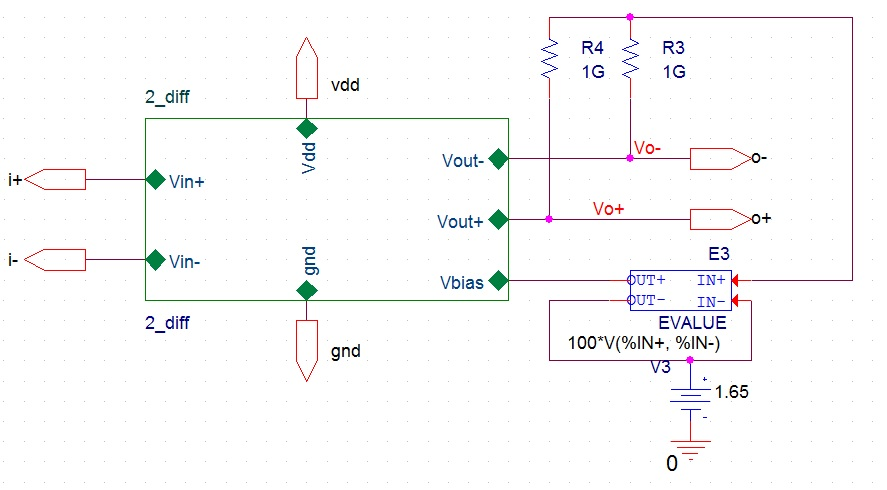
\includegraphics[width=\linewidth]{schema_rebouclage.png}

NB: l’élement «EVALUE» simule simplement un amplificateur idéal de 40 dB de gain centré sur 1.65V.

\section{Calcul de la capacité de compensation $C_C$ afin de stabiliser le circuit chargé par 2pF}

On trace le diagramme de Bode de la partie différentielle de l’amplificateur avec une capacité de
compensation de 5pF, ce qui permet d’avoir une marge de phase de 60°:

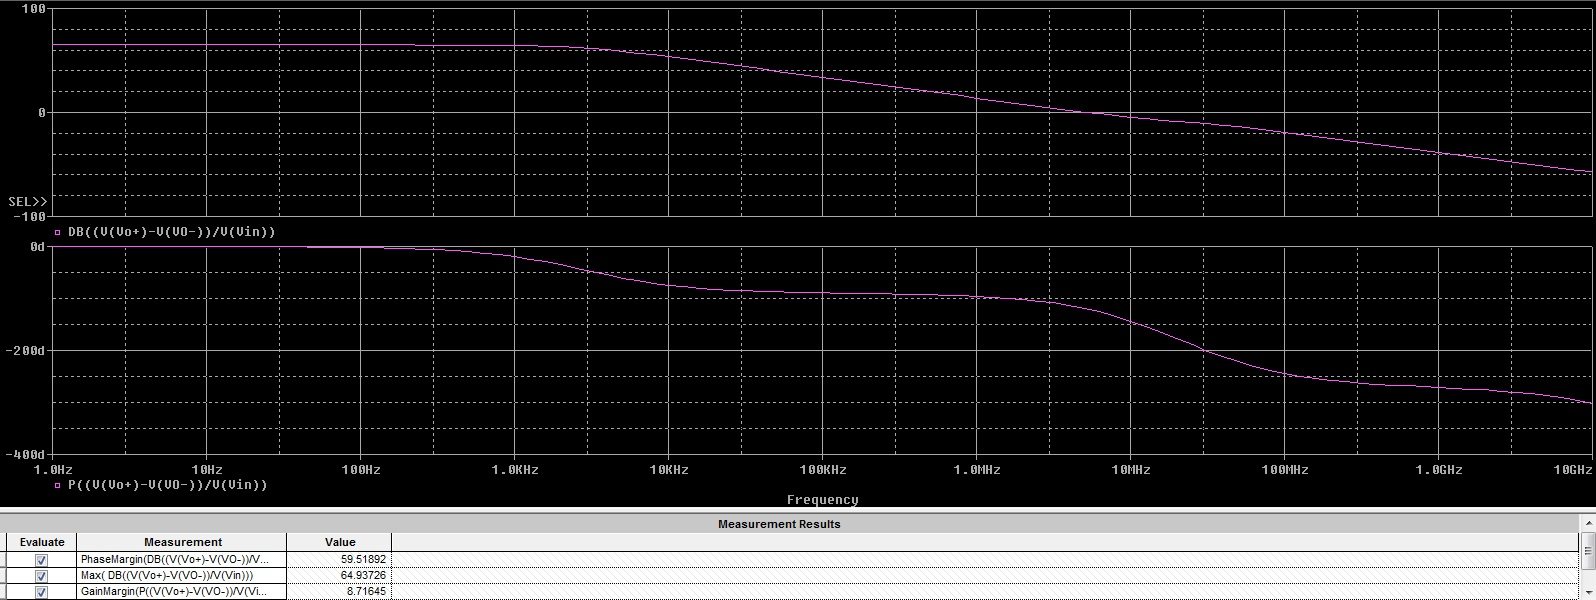
\includegraphics[width=\linewidth]{bode_diff_2p_load.png}

On observe une bande passante de l’ordre de 5kHz ; on choisira donc une fréquence de chopping de 1kHz.

\section{Conception du circuit de CMFB \& stabilité de la boucle}

On trace maintenant le diagramme de Bode du mode commun afin de vérifier qu’il soit suffisament rejeté:

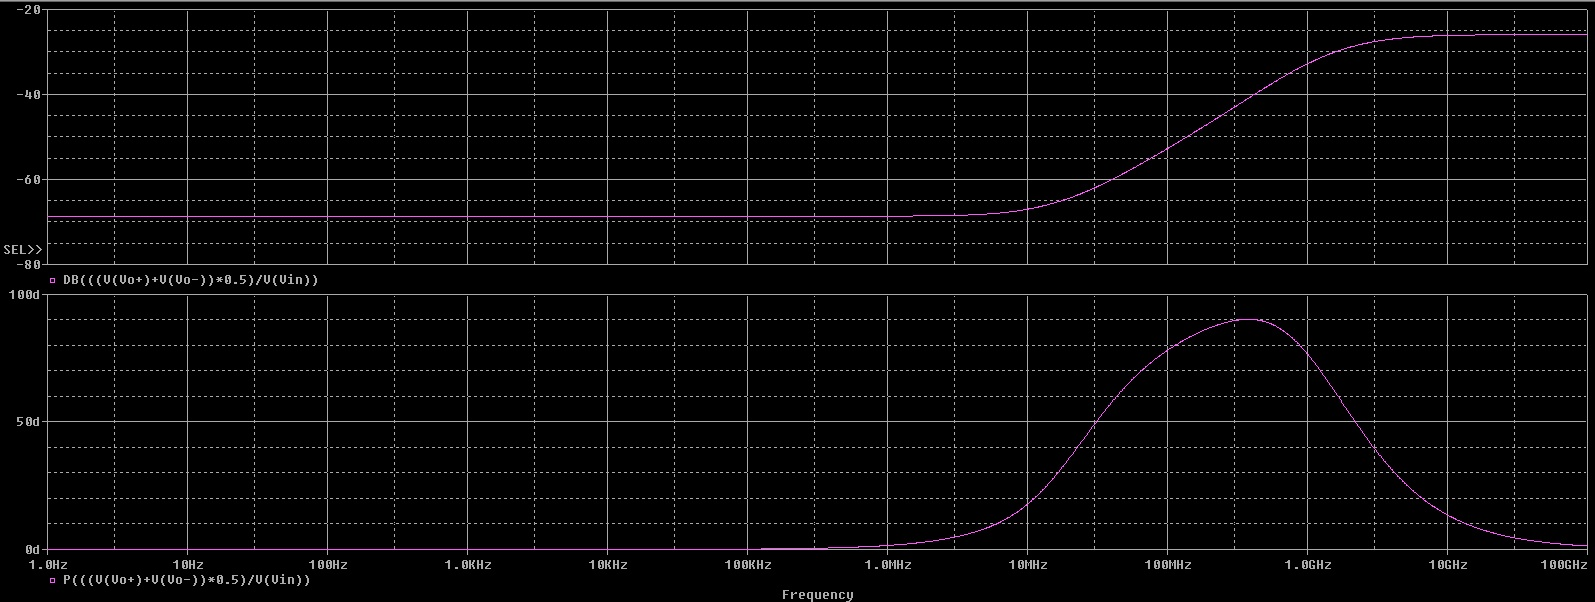
\includegraphics[width=\linewidth]{bode_mode_commun.png}

\newpage

\section{Diagramme de Bode de l’amplificateur différentiel et du CMFB}

Voici donc notre schéma final:

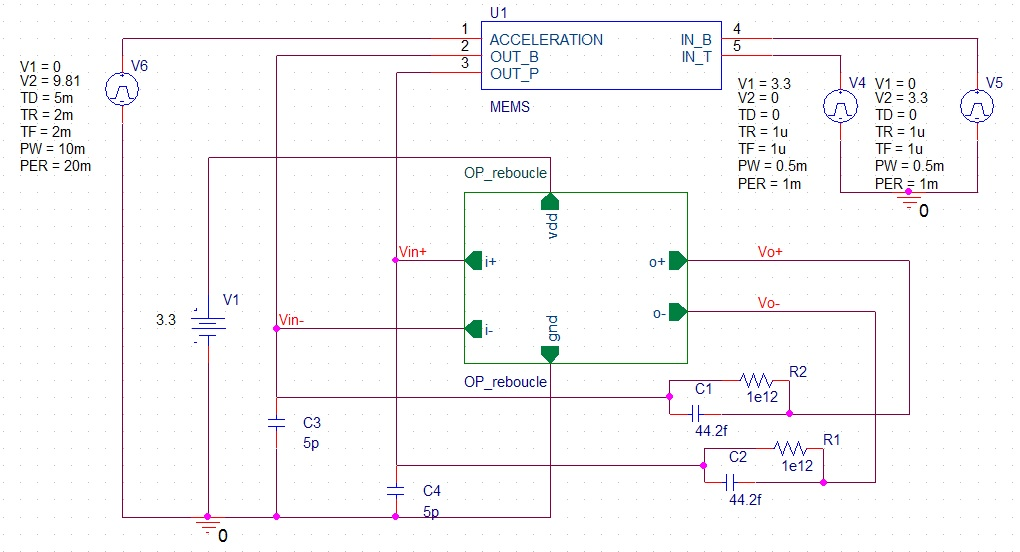
\includegraphics[width=\linewidth]{schema_final.jpg}

Et en simulation, on observe bien une tension d’un 1V pour une accélération d’1g.

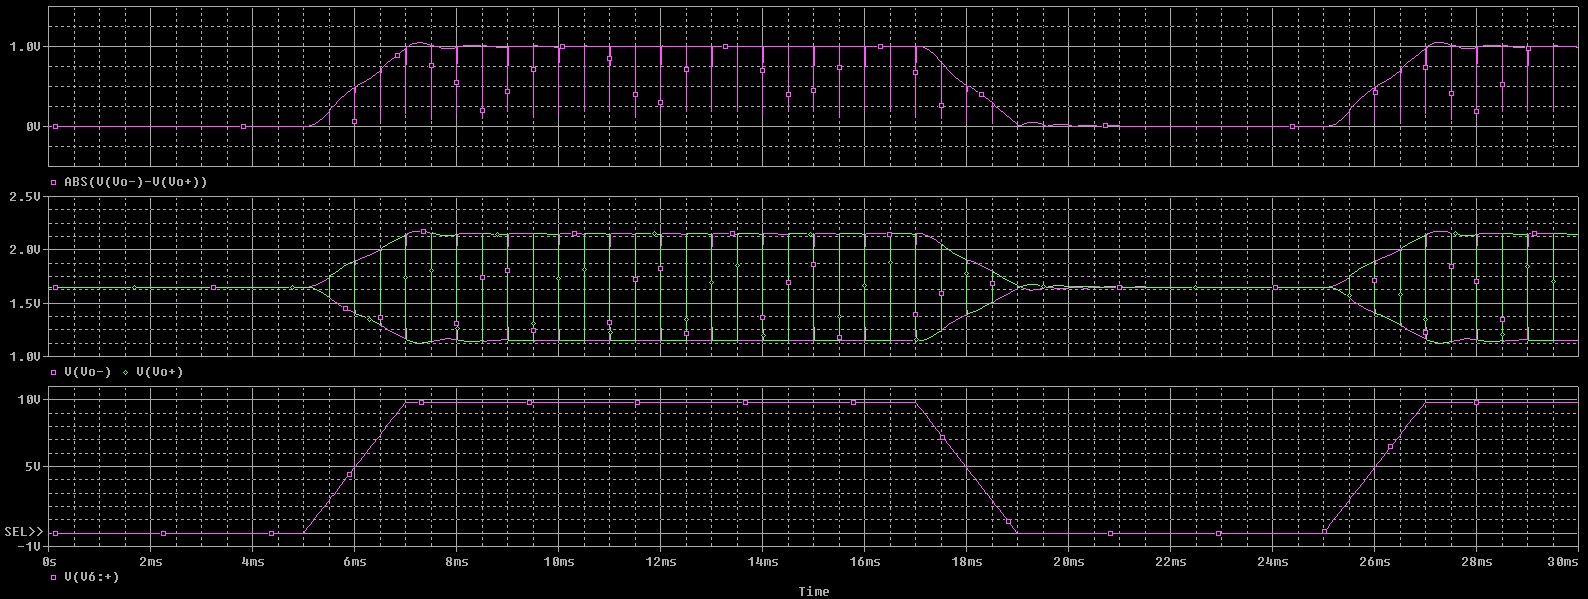
\includegraphics[width=\linewidth]{simulation_finale.jpg}

\newpage

\section*{Conclusion}

Ce projet nous a permis de voir à la fois une chaîne d’instrumentation et les techniques de mise en place d’un FDA et d’un CCMB.
Il était intéressant et ne semblait pas particulièrement difficile, surtout que nous avons clairement opté pour la solution la plus basique au niveau du CCMB.

~

Cependant, nous avons perdu un temps fou à plusieurs moments à cause de certains paramètres de simulation que nous ne maîtrisons toujours pas à la fin de cette troisième année, tels que, basiquement, le pas minimal de simulation. Nous sommes en effet tombés sur des cas où ne pas le spécifier faisait n’importe quoi, en spécifier un trop gros faisait n’importe quoi, et en spécifier un trop faible faisait n’importe quoi.

~

Et par «n’importe quoi», on veut dire à chaque fois un ou plusieurs de ces cas:

\begin{itemize}
    \item Le temps de simulation dépasse la dizaine de minutes;
    \item La simulation ne converge pas;
    \item La simulation semble converger au début, mais diverge au bout d’un temps aléatoire;
    \item Le résultat est aberrant.
\end{itemize}

~

Par exemple, ce suiveur:

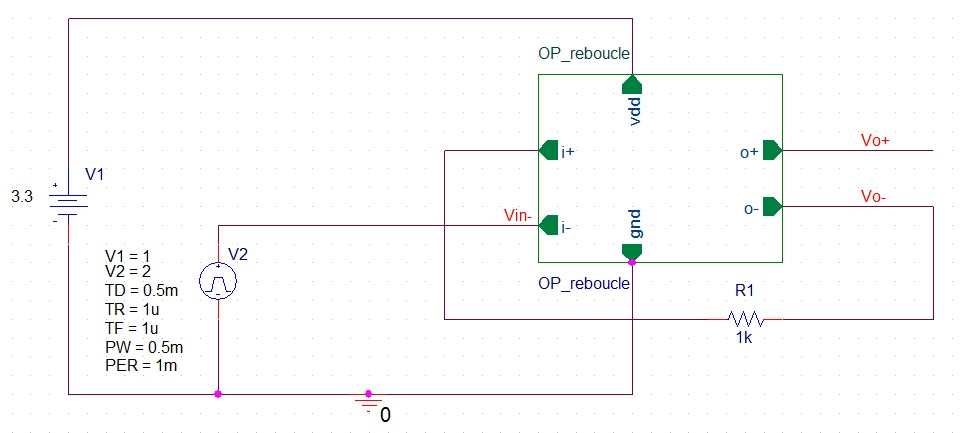
\includegraphics[width=\linewidth/2]{suiveur_schema.png}

donne ce qui est attendu avec un pas de 1µs:

%\begin{multicols}{2}

    %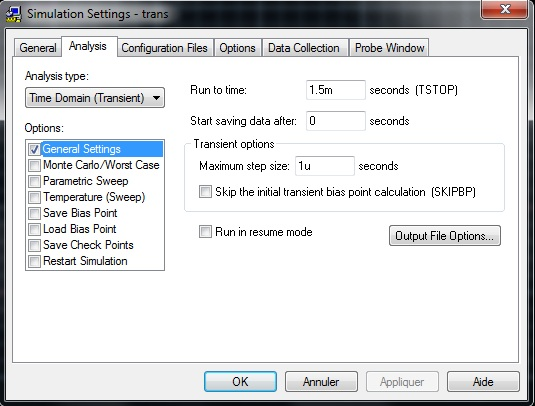
\includegraphics[width=\linewidth]{param_suiveur_qui_marche.png}

    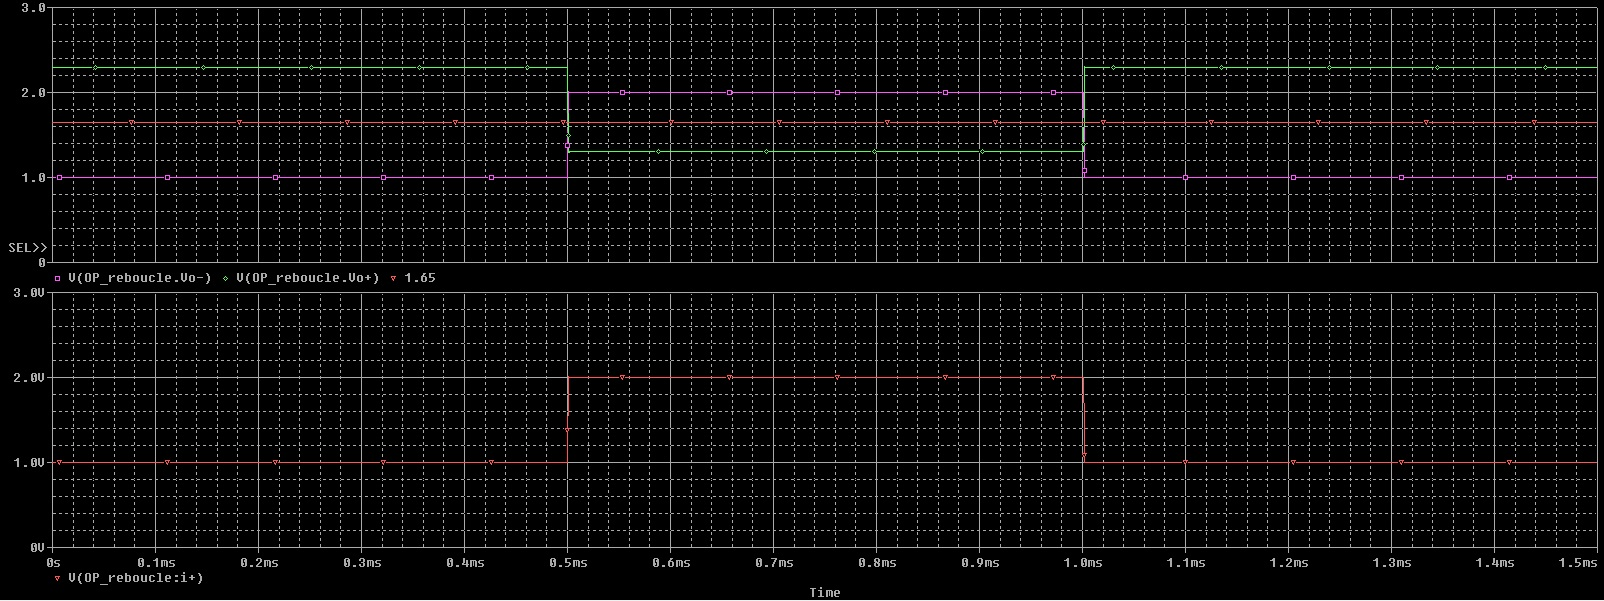
\includegraphics[width=\linewidth-3cm]{suiveur_qui_marche.png}

    %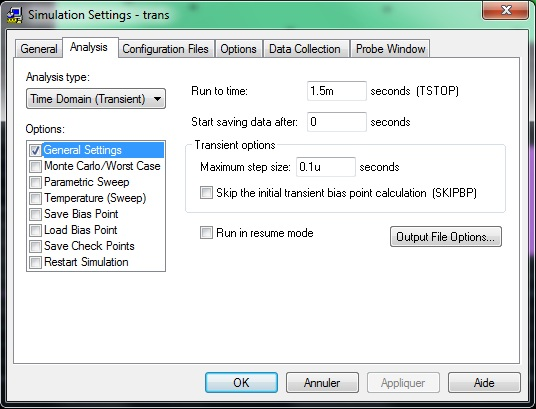
\includegraphics[width=\linewidth]{param_suiveur_qui_plante.png}
mais donne n’importe quoi pour un pas de 0.1µs:

    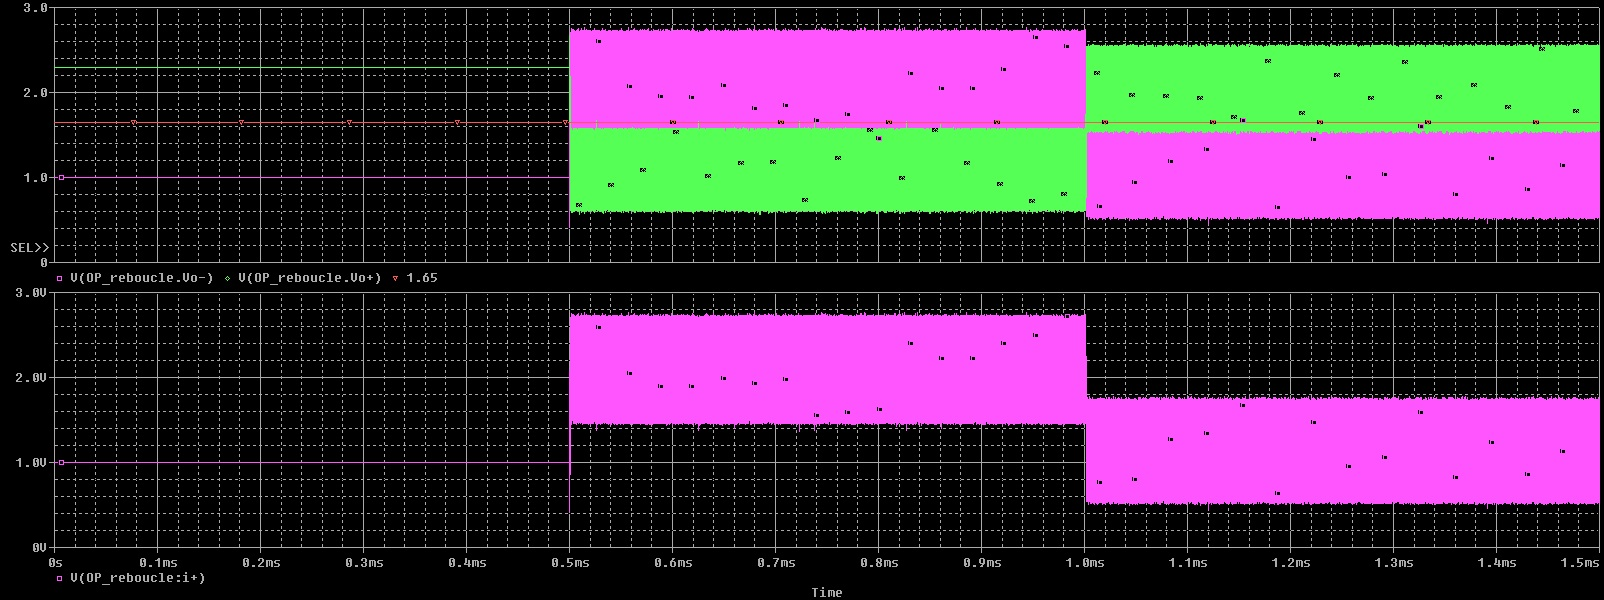
\includegraphics[width=\linewidth-3cm]{suiveur_qui_plante.png}

%\end{multicols}

\end{document}
